\part{Model Predictive Control}

\chapter{Linear Model Predictive Control}
\label{chap:linear_mpc}

\begin{quote}
	\textit{``MPC is like playing chess: you predict several moves ahead, pick the best move, execute it, and then -- because the opponent [uncertainty] might play differently than expected -- you re-evaluate the board and plan again.''} \\
	\hfill --- paraphrasing the receding horizon principle
\end{quote}

This chapter extends unconstrained optimal control (LQR) to handle physical limits. We define the Linear MPC problem, showing how actuator saturation and safety constraints are incorporated directly into the optimisation. We then cover the \emph{Receding Horizon} principle, introduce the \emph{YALMIP} toolbox for implementation, and analyse how the prediction horizon $N$ and the terminal cost $P$ affect closed-loop stability and performance.

\section{Motivation: The Need for Constraints}

In the previous chapters, we derived the Linear Quadratic Regulator (LQR). This method provides a closed-form solution to the optimal control problem, yielding a static feedback gain matrix $K$. However, LQR relies on a critical, often unrealistic assumption: \emph{the system operates in an unconstrained linear world.}

In physical reality, every engineering system has limits:
\begin{itemize}
	\item \textbf{Actuator Saturation:} A motor has a maximum voltage; a valve cannot open beyond 100\%.
	\item \textbf{Safety Constraints:} A chemical reactor must not exceed a critical pressure; a robotic arm must stay within a defined workspace.
	\item \textbf{Performance Bounds:} A passenger vehicle must limit acceleration to ensure comfort.
\end{itemize}

\subsection*{Why \emph{Clipping} in LQR Fails}
A common naive approach is to design an LQR controller and simply \emph{clip} or saturate the control signal if it exceeds the limit: 
\[ u = \text{sat}(-Kx) = \begin{cases}
	u_\text{max} & -Kx \ge u_\text{max} \\
	u_\text{min} & -Kx \le u_\text{min} \\
	-Kx & \text{otherwise}
\end{cases} \]
While this works for small disturbances, it breaks the mathematical guarantee of optimality and stability. Saturating the input effectively turns a linear system into a non-linear one. If the LQR controller requests a strong braking force to stabilise a fast-moving vehicle, but the actuator saturates, the vehicle may overshoot or become unstable because the "planned" energy dissipation did not occur.

\subsection*{From Offline Gains to Online Optimisation}
\emph{Model Predictive Control (MPC)} fundamentally alters this approach. Instead of calculating a control law \textit{offline} (like the LQR gain $K$), MPC solves a constrained optimisation problem \textit{online} at every time step.

By incorporating the constraints directly into the prediction model, MPC "knows" about the limits in advance. It does not blindly request impossible inputs; instead, it plans a trajectory that rides the very edge of the feasible region without crossing it. This capability—to operate safely and optimally against constraints—is what makes MPC the standard in advanced industrial control.

In this chapter, we will formulate the Linear MPC problem and demonstrate how to implement it efficiently using the YALMIP toolbox.

\section{Problem Formulation}
\label{sec:mpc_formulation}

The fundamental goal of MPC is to compute a sequence of future control inputs that drives the system state to the origin (or a target setpoint) whilst satisfying all physical constraints.

At every sampling instant $t$, we measure the current state of the system, denoted as $x(t)$. We then define an optimal control problem over a finite \emph{prediction horizon} of $N$ steps. To distinguish the prediction from the actual system evolution, we use the index $k$ to denote the steps into the future (where $k=0$ represents the current time $t$).

We solve the following constrained optimisation problem:

\begin{equation} \label{eq:mpc_cost}
	\min_{{u}, {x}} J = \underbrace{x_N^\top Q_N x_N}_{\text{Terminal Cost}} + \sum_{k=0}^{N-1} \left( \underbrace{x_k^\top Q x_k}_{\text{State Penalty}} + \underbrace{u_k^\top R u_k}_{\text{Control Effort}} \right)
\end{equation}

\textbf{Subject to:}
\begin{align*}
	\textbf{Initialisation:} \quad & x_0 = x(t) && (\text{Current measured state}) \\
	\textbf{Model Dynamics:} \quad & x_{k+1} = A x_k + B u_k, && k=0,\dots,N-1 \\
	\textbf{Actuator Limits:} \quad & u_{\min} \le u_k \le u_{\max}, && k=0,\dots,N-1 \\
	\textbf{Safety Limits:} \quad & x_{\min} \le x_k \le x_{\max}, && k=1,\dots,N
\end{align*}

Where:
\begin{itemize}
	\item ${u} = \{u_0, u_1, \dots, u_{N-1}\}$ is the sequence of future control inputs to be optimised.
	\item ${x} = \{x_1, x_2, \dots, x_N\}$ is the sequence of predicted states.
	\item $Q \succeq 0$ and $R \succ 0$ are the stage cost weighting matrices.
	\item $Q_N \succeq 0$ is the terminal weight, often chosen to approximate the infinite-horizon cost (i.e., the solution to the Riccati equation, $P$).
\end{itemize}

\section{The Receding Horizon Principle}
The defining feature of MPC is its \emph{Receding Horizon} strategy. Rather than computing a single fixed trajectory from start to finish, the controller operates in a loop:

\begin{enumerate}
	\item \textbf{Measure:} Obtain the current state $x(t)$.
	\item \textbf{Solve:} Compute the optimal sequence $\{u_0, u_1, \dots, u_{N-1}\}$ by solving the constrained optimisation problem (\ref{eq:mpc_cost}).
	\item \textbf{Apply:} Inject \emph{only the first input} $u_0$ into the system. The rest of the sequence is discarded.
	\item \textbf{Recede:} Wait for the next sampling instant $t+1$, measure the new state $x(t+1)$, and repeat the process.
\end{enumerate}

By re-solving the problem at every time step based on fresh measurements, the MPC converts an open-loop optimal plan into a \emph{closed-loop feedback strategy}, capable of rejecting disturbances and correcting model mismatches.

\begin{examplebox}{Hand-Worked MPC: Scalar Integrator with Constraints}
We now solve the MPC problem \emph{entirely by hand} to make the mechanics concrete before moving to MATLAB.

\textbf{System:}
\[
x_{k+1} = x_k + u_k \qquad \text{(pure integrator)}
\]
\textbf{Parameters:} $Q = 1$, $R = 1$, $Q_N = 1$, prediction horizon $N = 2$, input constraint $|u_k| \le 0.5$.

\textbf{Initial condition:} $x_0 = 1$.

\textbf{Step 1 --- Write the predicted states in terms of the decisions:}
\begin{align*}
x_1 &= x_0 + u_0 = 1 + u_0 \\
x_2 &= x_1 + u_1 = 1 + u_0 + u_1
\end{align*}

\textbf{Step 2 --- Substitute into the cost function:}
\begin{align*}
J &= \underbrace{x_0^2}_{=1} + u_0^2 + \underbrace{x_1^2}_{(1+u_0)^2} + u_1^2 + \underbrace{x_2^2}_{(1+u_0+u_1)^2}
\end{align*}
Expanding and collecting:
\[
J = 3 + 4u_0 + 2u_1 + 3u_0^2 + 2u_0 u_1 + 2u_1^2
\]
This is a quadratic in $u = [u_0 \;\; u_1]^\top$:
\[
J = u^\top \underbrace{\begin{bmatrix} 3 & 1 \\ 1 & 2 \end{bmatrix}}_{H} u + \underbrace{\begin{bmatrix} 4 \\ 2 \end{bmatrix}^\top}_{f^\top} u + 3
\]

\textbf{Step 3 --- Solve the unconstrained QP:}

Setting $\nabla_{u} J = 2Hu + f = 0$:
\[
u^\star = -\tfrac{1}{2}H^{-1}f = -\frac{1}{2} \cdot \frac{1}{5}\begin{bmatrix} 2 & -1 \\ -1 & 3 \end{bmatrix}\begin{bmatrix} 4 \\ 2 \end{bmatrix} = -\frac{1}{10}\begin{bmatrix} 6 \\ 2 \end{bmatrix} = \begin{bmatrix} -0.6 \\ -0.2 \end{bmatrix}
\]

\textbf{Step 4 --- Check constraints:}

Since $|u_0^\star| = 0.6 > 0.5$, the constraint is violated. We set $u_0 = -0.5$ (at its bound) and re-optimise over $u_1$ alone:
\[
x_1 = 1 - 0.5 = 0.5, \qquad x_2 = 0.5 + u_1
\]
\[
J(u_1) = u_1^2 + (0.5 + u_1)^2 + \text{const.} = 2u_1^2 + u_1 + \text{const.}
\]
\[
\frac{dJ}{du_1} = 4u_1 + 1 = 0 \quad\Longrightarrow\quad u_1^\star = -0.25 \quad (\text{feasible})
\]

\begin{notebox}{Note on constraint handling}
The manual approach above --- fixing the active constraint and solving the remaining subproblem --- is illustrative but does not generalise to higher dimensions. In practice, QP solvers use active-set or interior-point methods to handle constraints systematically.
\end{notebox}

\textbf{Step 5 --- Apply the Receding Horizon:}

We apply \emph{only} $u_0^\star = -0.5$ and \emph{discard} $u_1^\star = -0.25$.

The plant advances: $x_1 = 0.5$. We now re-measure and re-solve with $x_0 = 0.5$.

Since the problem is linear in $x_0$, the new unconstrained solution scales:
$u^\star = 0.5 \times [-0.6,\; -0.2]^\top = [-0.3,\; -0.1]^\top$. Both inputs satisfy $|u_k| \le 0.5$, so the constraints are inactive. We apply $u_0 = -0.3$ and the state moves to $x_1 = 0.2$.

\textbf{Summary of the closed-loop trajectory:}
\begin{center}
\begin{tabular}{cccc}
\toprule
Step $t$ & $x(t)$ & $u^\star_0$ & Constraint active? \\
\midrule
0 & 1.0  & $-0.50$ & Yes \\
1 & 0.50 & $-0.30$ & No \\
2 & 0.20 & $-0.12$ & No \\
3 & 0.08 & $\cdots$ & No \\
\bottomrule
\end{tabular}
\end{center}

\textbf{Key observations:}
\begin{enumerate}[noitemsep]
\item The constraint is active only at the first step, when the state is large. As $x$ shrinks, the problem becomes unconstrained and the MPC law approaches the LQR law.
\item Only the first input is ever applied --- re-planning at each step provides feedback.
\item The QP matrices $H$ and $f$ are fixed; only $f$ changes with $x_0$. This is why the \texttt{optimizer} object in the next section treats $x_0$ as a parameter.
\end{enumerate}
\end{examplebox}

\section{Efficient Implementation via YALMIP}

To implement MPC, we utilise \emph{YALMIP}~\cite{Lofberg2004}, a MATLAB toolbox that allows us to define optimisation problems using high-level symbolic code.

A naive implementation would define and solve the problem from scratch inside the simulation loop. This is computationally prohibitive because YALMIP would need to re-parse the mathematical structure every few milliseconds. Instead, we use a technique known as \emph{Parametric Programming}.

We construct the problem \emph{once} offline, treating the initial state $x_0$ as a symbolic \emph{parameter}. The YALMIP \texttt{optimizer} object then maps this parameter to the optimal decision variables, allowing for extremely fast execution during the simulation.

\section{Stability and the Terminal Cost}
Before writing the code that solves standard MPC, we must ensure stability~\cite{Mayne2000}. For a finite horizon $N$, MPC is not automatically guaranteed to stabilise the system. To address this, we include a \emph{Terminal Cost} weighted by a matrix $Q_N$:
\begin{equation*}
	J_{term} = x_N^\top Q_N x_N
\end{equation*}

\begin{alertbox}{Selection of the terminal weight $Q_N$}
Choosing the terminal weight as
\[
Q_N = P,
\]
where \(P\) is the positive semidefinite solution of the discrete algebraic Riccati equation
\[
P = A^\top P A - A^\top P B (R + B^\top P B)^{-1} B^\top P A + Q,
\]
is a natural and important choice because it matches the infinite-horizon LQR cost-to-go. In the unconstrained case, this choice makes the finite-horizon MPC law consistent with the LQR solution near the origin. 

In the constrained case, however, the terminal cost \(P\) alone does not in general guarantee closed-loop stability for arbitrary horizon lengths. A rigorous stability guarantee typically also requires a suitable terminal set and a terminal control law such that, inside the terminal set, the constraints remain satisfied and the terminal cost decreases under the terminal controller. Therefore, \(Q_N=P\) should be viewed as an essential stabilising ingredient, but not as a complete stability guarantee by itself unless the unconstrained LQR tail is known to be feasible.
\end{alertbox}


\subsection{The YALMIP Workflow}
The following script demonstrates the complete setup. Note that MATLAB uses 1-based indexing, so the symbolic variable \texttt{x\{k\}} corresponds to the mathematical state $x_{k-1}$.

\begin{lstlisting}[language=Matlab, caption={Efficient MPC setup using the YALMIP \texttt{optimizer} object.}, label={lst:yalmip_mpc}]
	% 1. Define Model and Parameters
	A = [1.1 1; 0 1]; B = [0; 1]; % Example System
	nx = 2; nu = 1;
	N = 10;                       % Prediction Horizon
	
	% 2. Weights and Constraints
	Q = eye(nx); R = 0.1;
	[P, ~, ~] = dare(A, B, Q, R); % Terminal Weight (Stability)
	u_max = 1; x_max = 5;
	u_min = -1; x_min = -5;
	
	% 3. Define Symbolic Variables
	% u(:,k) represents input u_{k-1}
	% x(:,k) represents state x_{k-1}
	u = sdpvar(nu, N);    
	x = sdpvar(nx, N+1);  
	
	% 4. Build Objective and Constraints Loop
	constraints = [];
	objective = 0;
	
	for k = 1:N
		% Stage Cost
		objective = objective + x(:,k)'*Q*x(:,k) + u(:,k)'*R*u(:,k);
		
		% Dynamics Constraint: x_{k} = A*x_{k-1} + B*u_{k-1}
		constraints = [constraints, x(:,k+1) == A*x(:,k) + B*u(:,k)];
		
		% Physical Constraints
		constraints = [constraints, u_min <= u(:,k) <= u_max];
		constraints = [constraints, x_min <= x(:,k) <= x_max];
	end
	
	% Terminal Cost (The "Anchor" for stability)
	objective = objective + x(:,N+1)'*P*x(:,N+1);
	
	% 5. Create the Optimizer Object
	% We treat the 'current state' (x(:,1)) as a PARAMETER.
	% The solver will return the 'first input' (u(:,1)).
	parameters_in = x(:,1);
	solutions_out = u(:,1);

	opts = sdpsettings('verbose', 0, 'solver', 'quadprog');
	controller = optimizer(constraints, objective, opts, parameters_in, solutions_out);
	
	% --- SIMULATION USAGE ---
	% Inside the simulation loop, we simply call:
	% u_optimal = controller(x_current);
\end{lstlisting}

\begin{notebox}{Indexing Alert}
	Pay close attention to indexing. In mathematics, we start at $k=0$ (current state). In MATLAB, indices start at 1. Therefore:
	\begin{itemize}
		\item Math $x_0$ $\rightarrow$ Code \texttt{x(:,1)} (The Parameter)
		\item Math $u_0$ $\rightarrow$ Code \texttt{u(:,1)} (The Output to apply)
		\item Math $x_N$ $\rightarrow$ Code \texttt{x(:,N+1)} (The Terminal State)
	\end{itemize}
\end{notebox}

\begin{examplebox}{MATLAB: Full MPC Simulation with YALMIP}
	\textbf{System Definition:}
	We consider a discrete-time linear system with unstable and oscillatory dynamics. The state-space matrices are:
	\begin{equation*}
		A = \begin{bmatrix} 1.5 & 0 \\ 1 & -1.5 \end{bmatrix}, \quad B = \begin{bmatrix} 1 \\ 0 \end{bmatrix}
	\end{equation*}
	Note that the eigenvalue $\lambda = -1.5$ introduces a discrete-time oscillation (sign flipping at every step) combined with unstable growth, making this a challenging control target.
	
	\textbf{The MPC Optimisation Problem:}
	At each sampling instant, the controller solves the following quadratic programme (i.e.\ an optimisation problem with a quadratic cost function and linear constraints) with a prediction horizon of $N=5$:
	
	\begin{equation*}
		\min_{u_0, \dots, u_{N-1}} J = x_N^\top P x_N + \sum_{k=0}^{N-1} \left( x_k^\top Q x_k + u_k^\top R u_k \right)
	\end{equation*}
	where $P$ is the LQR solution of the discrete-time Riccati equation.
	
	\textbf{Subject to:}
	\begin{align*}
		x_{k+1} &= A x_k + B u_k & \text{(Dynamics)}\\
		-5 &\leq u_k \leq 5 & \text{(Input Saturation)}\\
		\begin{bmatrix} -10 \\ -10 \end{bmatrix} &\leq x_k \leq \begin{bmatrix} 10 \\ 10 \end{bmatrix} & \text{(State Safety)}\\
		x_0 &= x(t) & \text{(Measurement)}
	\end{align*}
	
	\textbf{Parameters:}
	\begin{itemize}
		\item \textbf{Weights:} $Q = I_2$, $R = 20$. The high input cost $R$ penalises aggressive control actions.
		\item \textbf{Terminal Cost:} $P_N$ is the unique positive-definite solution to the unconstrained LQR Algebraic Riccati Equation.
	\end{itemize}
	Figure~\ref{fig:simplempc} shows the simulation result obtained after using the code provided below.
	\begin{lstlisting}[language=Matlab]
		% 1. System Matrices & MPC Weights
		A = [1.5 0; 1 -1.5];  B = [1; 0];
		nx = 2; nu = 1;
		Q = eye(2); R = 20;
		
		[P,~,~] = dare(A,B,Q,R);
		
		u_min = -5; u_max = 5;
		x_min = [-10; -10]; x_max = [10; 10];
		
		N = 5;
		
		% 2. YALMIP Formulation
		u = sdpvar(nu, N);
		x = sdpvar(nx, N+1);
		x_init = sdpvar(nx, 1);
		
		obj = 0; 
		cons = [x(:,1) == x_init];
		
		for k = 1:N
				obj = obj + x(:,k)'*Q*x(:,k) + u(:,k)'*R*u(:,k);
				cons = [cons, x(:,k+1) == A*x(:,k) + B*u(:,k)];
				cons = [cons, u_min <= u(:,k) <= u_max];
				cons = [cons, x_min <= x(:,k) <= x_max];
		end
		
		obj = obj + x(:,N+1)'*P*x(:,N+1);
		
		% 3. Optimizer
		opts = sdpsettings('verbose', 0, 'solver', 'quadprog');
		mpc_controller = optimizer(cons, obj, opts, x_init, u(:,1));
		
		% 4. Simulation Loop
		T_sim = 30;
		x_state = [1; -2]; % Initial Condition
		
		% Initialize History arrays
		x_hist = zeros(nx, T_sim+1); 
		u_hist = zeros(nu, T_sim);
		
		% Save the initial state at index 1 (Time 0)
		x_hist(:,1) = x_state;
		
		for t = 1:T_sim
				% A. Solve MPC
				[u_opt, errorcode] = mpc_controller(x_state);
		
				if errorcode ~= 0, 
					warning('Solver failed!'); 
				end
		
				% B. Log Control (at time k)
				u_hist(:,t) = u_opt;
		
				% C. Apply Control / Plant Physics
				x_state = A*x_state + B*u_opt;
		
				% D. Log Next State (at time k+1)
				x_hist(:,t+1) = x_state;
		end
		
		% 5. Plotting
		t_vec_x = 0:T_sim;    % State time vector (0 to 30)
		t_vec_u = 0:T_sim-1;  % Control time vector (0 to 29)
		
		figure;
		subplot(2,1,1);
		plot(t_vec_x, x_hist(1,:), 'LineWidth', 2); hold on;
		plot(t_vec_x, x_hist(2,:), 'LineWidth', 2); 
		grid on;
		ylabel('Position'); title('State Regulation');
		legend('x_1', 'x_2');
		xlim([0 T_sim]);
		
		subplot(2,1,2);
		stairs(t_vec_u, u_hist(1,:), 'LineWidth', 2); hold on; 
		yline(u_max, 'r--', 'Max Limit', 'LineWidth', 2);
		yline(u_min, 'r--', 'Min Limit', 'LineWidth', 2);
		ylabel('Control Input (u)'); grid on;
		xlabel('Time Steps');
		xlim([0 T_sim]);
	\end{lstlisting}


	\begin{center}
	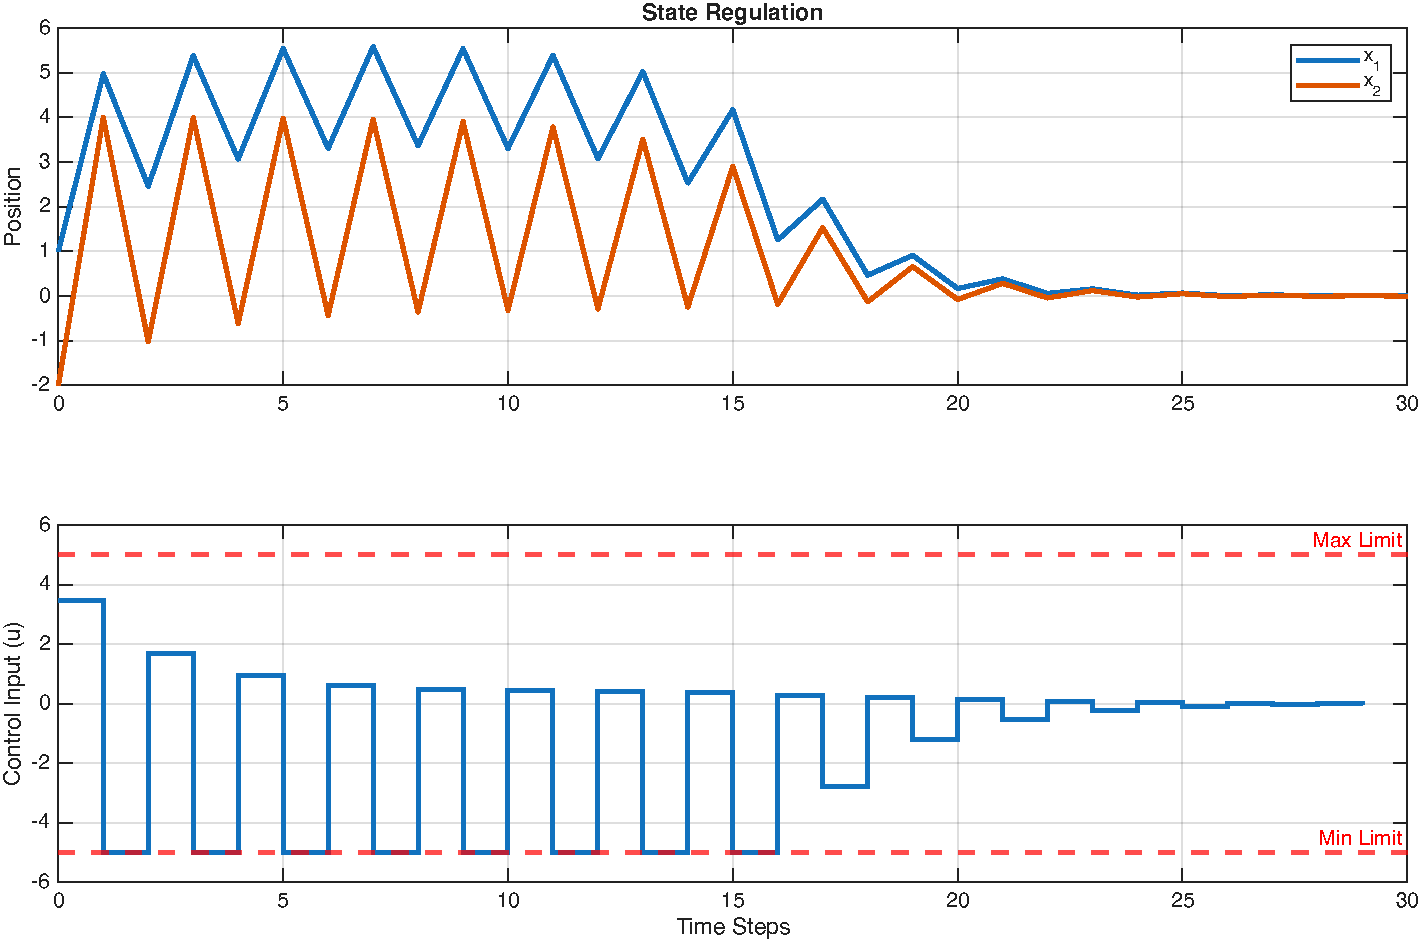
\includegraphics[width=0.7\linewidth]{Figures/Simple_MPC}
	\captionof{figure}{\emph{MPC Regulation of an Unstable Oscillatory System.}
		The top plot displays the state trajectories starting from $x_0 = [1; -2]^\top$. The characteristic "zig-zag" behaviour is caused by the negative eigenvalue $\lambda = -1.5$, while the instability drives the amplitude growth. 
		The bottom plot shows the control effort. The MPC controller effectively "clamps" the input to the constraint boundary ($u_{\min} = -5$) for the first 16 steps to counteract the unstable dynamics. Once the system energy is sufficiently reduced (around $t=18$), the control signal enters the linear region and smoothly drives the states to the origin.}
	\label{fig:simplempc}
\end{center}

\end{examplebox}

\section{The Effect of Horizon ($N$) and Terminal Cost ($P$)}
\label{sec:effect_of_N}

A common pitfall in MPC design is choosing parameters that make the controller "myopic" (short-sighted). If the horizon $N$ is too short, the controller may not see the approaching constraints or the equilibrium point in time to stop, leading to instability.

We can solve this problem in two ways:
\begin{enumerate}
	\item \textbf{Increase $N$:} This extends the controller's vision, but increases computational complexity linearly (or polynomially, depending on the solver). Typically it would be reasonable to choose 
	\begin{equation*}
		N \cdot T_s \approx T_\text{settling}
	\end{equation*}
	This selection is dependent on $T_\text{sampling}$. 	In other words, we aim to have approximately $10$ to $20$ samples during the rising phase of the step response:
	\begin{equation*}
		T_\text{sampling} \approx \frac{T_r}{10} \quad \text{to} \quad \frac{T_r}{20}
	\end{equation*}
	where $T_r$ is the rise time of the system that is controlled. Hence, 
		\begin{equation*}
		N \approx 20 \text{--} 50 \text{ samples}
	\end{equation*}

	\item \textbf{Add Terminal Cost $P$:} This adds an "artificial" cost to the end of the horizon. By setting $P$ equal to the infinite-horizon LQR cost, we trick the controller into thinking it plans for eternity, even if $N$ is small.
\end{enumerate}

While short horizons can lead to instability, a more common issue in practice is \emph{Performance Degradation}. If the control authority is "expensive" (high $R$) and the horizon is short, the controller becomes "lazy."

\begin{figure}[h]
	\centering
	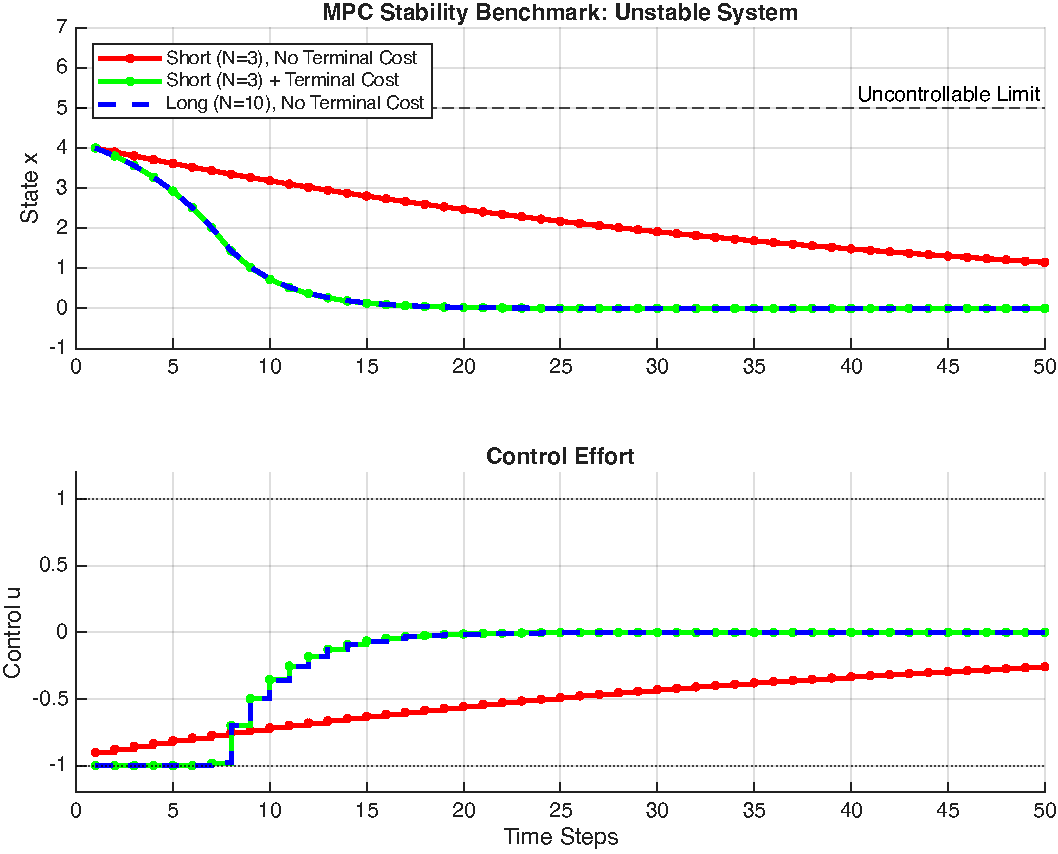
\includegraphics[width=0.9\linewidth]{Figures/Effect_of_N.pdf} 
	\caption{\emph{Performance Degradation with Short Horizons.} The system starts at $x_0=4$ with expensive control ($R=10$). The Short Horizon controller (Red) tries to save control effort in the short term as it cannot see long enough, leading to extremely slow convergence. The Terminal Cost controller (Green) recognises the long-term value of aggressive action, matching the performance of the Long Horizon controller (Blue).}
	\label{fig:mpc_lazy}
\end{figure}

\begin{examplebox}{MATLAB Benchmark: Stability Analysis}
	To rigorously test the stability properties of the MPC controller, we utilise an \emph{open-loop unstable scalar system}.
	
	\textbf{1. The Experiment:}
	We define an unstable system subject to strict input constraints:
	\begin{equation*}
		x_{k+1} = 1.2 x_k + u_k, \qquad -1 \leq u_k \leq 1
	\end{equation*}
	The initial condition $x_0 = 4$ is chosen close to the controllability limit. We compare three controller configurations:
	\begin{enumerate}
		\item \textbf{Short Horizon ($N=3$):} A very myopic controller.
		\item \textbf{Long Horizon ($N=10$):} A far-sighted controller.
		\item \textbf{Short Horizon with $P$ ($N=3, P=P_{LQR}$):} A myopic controller compensated with a terminal cost.
	\end{enumerate}
	
	\textbf{2. The Results (see Figure \ref{fig:mpc_lazy}):}
	\begin{itemize}
		\item \textbf{The Lazy Controller (Red Line):} 
		With $N=3$ and no terminal cost, the controller minimises the cost over a very short window. It calculates that applying maximum braking ($u=-1$) is \emph{too expensive} ($R=10$) relative to the short-term reduction in state error. It chooses a "soft" braking strategy ($u \approx -0.9$). While this prevents immediate explosion, convergence is very slow. The controller fails to realise that dragging out the error over a long time will result in a much higher \textit{total} cost.
		
		\item \textbf{The Optimal Controller (Green/Blue Lines):} 
		By adding the Terminal Cost ($P$) or extending the horizon ($N=10$), the controller accounts for the \emph{infinite tail} of the cost function. It realises that while braking hard ($u=-1$) is expensive \textit{now}, it is the only way to minimise the sum of squared errors over the long run. Consequently, it acts aggressively, driving the state to zero in minimal time.
	\end{itemize}
	
	\textbf{Conclusion:} The Terminal Cost $P$ is not just a stability anchor; it is a crucial tuning parameter that restores \emph{long-term optimality} to short-horizon controllers.
\end{examplebox}

% ================================================================
% FORMAL STABILITY THEORY
% ================================================================
\section{Recursive Feasibility and Formal Stability Guarantees\texorpdfstring{$^{(*)}$}{(*)}}
\label{sec:mpc_stability_theory}

The previous sections showed experimentally that adding the terminal cost $P$ improves MPC performance and can prevent instability. We now explain \textit{why} this works, and what additional ingredient is needed to \textit{guarantee} stability rigorously.

\subsection{The Gap in the Argument}

Consider the MPC cost function:
\[
J = \sum_{k=0}^{N-1} \bigl(x_k^\top Q\, x_k + u_k^\top R\, u_k\bigr) + x_N^\top P\, x_N
\]
The terminal cost $x_N^\top P\, x_N$ is supposed to represent the cost of controlling the system from $x_N$ to the origin \textit{after} the horizon ends. This representation is exact when the LQR controller $u = -Kx$ is applied from step $N$ onward \emph{and no constraints are violated} during that infinite tail.

But nothing in the formulation above prevents $x_N$ from landing in a region where the LQR input $-Kx_N$ would violate the constraint $|u| \le u_{\max}$. If that happens, the terminal cost $P$ is wrong --- it promises a future cost that cannot actually be achieved without breaking the constraints.

This is not only a theoretical concern. When $x_N$ is large and the constraints are tight, the MPC may plan a trajectory that looks optimal over the $N$-step window but leads to constraint violations (or solver infeasibility) at the very next time step.

To close this gap, we need two things:
\begin{enumerate}
	\item A \emph{terminal set} $\mathcal{X}_f$ --- a region of the state space where the LQR controller can operate indefinitely without violating any constraint.
	\item A \emph{terminal constraint} $x_N \in \mathcal{X}_f$ added to the MPC optimisation, which forces the predicted terminal state to land inside this safe region.
\end{enumerate}

\subsection{Positive Invariant Sets}

The terminal set $\mathcal{X}_f$ must have a very specific property: once the state enters $\mathcal{X}_f$, the LQR controller must keep it there forever, while satisfying all constraints at every future step. A set with this property is called \emph{positively invariant}.

\begin{defnbox}{Definition: Positive Invariant Set}
	A set $\mathcal{X}_f \subseteq \mathbb{R}^n$ is a \emph{positive invariant set} for the closed-loop system $x_{k+1} = (A - BK)\,x_k$ under the terminal control law $u = -Kx$, subject to constraints $u \in \mathcal{U}$, $x \in \mathcal{X}$, if for every state $x \in \mathcal{X}_f$ the following three conditions hold:
	\begin{enumerate}[noitemsep]
		\item The input $u = -Kx$ satisfies the input constraints: $-Kx \in \mathcal{U}$.
		\item The next state satisfies the state constraints: $(A - BK)x \in \mathcal{X}$.
		\item The next state stays in the set: $(A - BK)x \in \mathcal{X}_f$.
	\end{enumerate}
\end{defnbox}

Think of $\mathcal{X}_f$ as a \textit{safe harbour}. The MPC controller must steer the state into $\mathcal{X}_f$ by the end of the prediction horizon. Once the state is inside, the LQR controller takes over and handles everything from that point on --- no constraint violations, no instability, guaranteed convergence to the origin.

\subsection{Computing $\mathcal{X}_f$: A Scalar Example}
\label{subsec:terminal_set_scalar}

We compute $\mathcal{X}_f$ step by step for the scalar system used throughout this chapter.

\textbf{System:} $x_{k+1} = 1.2\,x_k + u_k$, with input constraint $|u_k| \le 1$.

\textbf{Step 1 --- Find the LQR gain.}
Solving the DARE with $Q = 1$, $R = 1$ gives $P \approx 1.95$ and:
\[
K = \frac{a P b}{R + b^2 P} = \frac{1.2 \times 1.95}{1 + 1.95} \approx 0.79
\]
The terminal controller is $u = -Kx \approx -0.79\,x$, and the closed-loop eigenvalue is:
\[
a_{cl} = a - bK = 1.2 - 0.79 = 0.41
\]
Since $|0.41| < 1$, the closed-loop system under LQR is stable.

\textbf{Step 2 --- Find the largest interval where the input constraint holds.}
The LQR input is $u = -Kx$. The constraint $|u| \le 1$ becomes $|Kx| \le 1$, which gives:
\[
|x| \le \frac{1}{K} = \frac{1}{0.79} \approx 1.27
\]
So the candidate terminal set is $\mathcal{X}_f = \{x : |x| \le 1.27\}$.

\textbf{Step 3 --- Verify positive invariance.}
Take any $x$ inside $\mathcal{X}_f$, so $|x| \le 1.27$. Under the LQR controller, the next state is:
\[
|x^+| = |a_{cl} \cdot x| = 0.41 \times |x| \le 0.41 \times 1.27 = 0.52
\]
Since $0.52 < 1.27$, the next state is well inside $\mathcal{X}_f$. The set is positively invariant.

In fact, the state \textit{contracts} by a factor of $0.41$ at each step inside $\mathcal{X}_f$. After entering the safe harbour, the system converges to zero quickly under the LQR controller.

\begin{notebox}{Why does this work?}
	The key is that the closed-loop eigenvalue satisfies $|a_{cl}| < 1$. This means $|x^+| < |x|$ for any non-zero $x$, so the state always shrinks. And because the boundary of $\mathcal{X}_f$ is defined by the constraint $|Kx| = 1$, the shrinking state can never reach the boundary again once it moves inward. The constraints remain satisfied at every future step.

	If the system also had state constraints $|x| \le x_{\max}$, we would need $\mathcal{X}_f \subseteq \{x : |x| \le x_{\max}\}$. For the example above, $1.27 < x_{\max}$ is required.
\end{notebox}

\subsection{The Complete MPC Problem with Terminal Constraint}

We now modify the MPC formulation from Section~\ref{sec:mpc_formulation} by adding the terminal constraint. The optimisation becomes:

\begin{align*}
	\min_{u} \quad & J = x_N^\top P\, x_N + \sum_{k=0}^{N-1} \bigl(x_k^\top Q\, x_k + u_k^\top R\, u_k\bigr) \\
	\text{s.t.} \quad & x_{k+1} = Ax_k + Bu_k, \quad k = 0, \ldots, N-1 \\
	& u_{\min} \le u_k \le u_{\max}, \quad k = 0, \ldots, N-1 \\
	& x_{\min} \le x_k \le x_{\max}, \quad k = 1, \ldots, N \\
	& {x_N \in \mathcal{X}_f}
\end{align*}

The only difference from before is the last line. This extra constraint restricts where the prediction horizon is allowed to end. The QP becomes slightly more constrained, but in return it provides a formal stability guarantee.

For the scalar case, $x_N \in \mathcal{X}_f$ simply means $|x_N| \le 1/K$. For multi-state systems, $\mathcal{X}_f$ is typically a polytope (a region defined by linear inequalities), and the constraint $x_N \in \mathcal{X}_f$ adds a set of linear inequalities to the QP --- so it remains a QP.

\subsection{Recursive Feasibility}

A controller is useless if it can solve the optimisation at time $t$ but not at time $t+1$. We need the guarantee that once the MPC problem is feasible, it \textit{stays} feasible forever. This property is called \emph{recursive feasibility}.

\begin{defnbox}{Definition: Recursive Feasibility}
	The MPC problem is \emph{recursively feasible} if, whenever a feasible solution exists at time $t$, a feasible solution also exists at time $t+1$ after applying the optimal input $u_0^\star$ to the plant.
\end{defnbox}

The proof uses a simple but powerful idea called the \emph{shifted sequence}.

\textbf{Setup.} Suppose at time $t$, the MPC solver returns the optimal input sequence:
\[
u^\star = \{u_0^\star,\; u_1^\star,\; \ldots,\; u_{N-1}^\star\}
\]
with predicted states $\{x_0, x_1, \ldots, x_N\}$, where $x_N \in \mathcal{X}_f$ (the terminal constraint is satisfied).

We apply $u_0^\star$ to the plant. The system moves to $x_1$.

\textbf{Constructing a feasible candidate at time $t+1$.}
At the next time step, we need \textit{some} feasible input sequence starting from $x_1$. We do not need the optimal one --- any feasible sequence proves that the problem has a solution. The optimiser will then find an even better one.

Here is our candidate:
\[
\tilde{u} = \{u_1^\star,\; u_2^\star,\; \ldots,\; u_{N-1}^\star,\; \underbrace{-K x_N}_{\text{LQR input at } x_N}\}
\]
We take the old optimal sequence, drop $u_0^\star$ (already used), shift everything one step to the left, and append the LQR input $-Kx_N$ at the end.

\textbf{Why is this candidate feasible?}
\begin{itemize}
	\item \textbf{Inputs $u_1^\star, \ldots, u_{N-1}^\star$:} These satisfied the constraints in the original problem, so they still do.
	\item \textbf{Predicted states $x_2, x_3, \ldots, x_N$:} These are the same states from the original prediction (the dynamics are deterministic). They satisfied the state constraints before, so they still do.
	\item \textbf{The appended input $-Kx_N$:} Since $x_N \in \mathcal{X}_f$ and $\mathcal{X}_f$ is positively invariant, the LQR input $-Kx_N$ satisfies the input constraints (by condition 1 of the definition).
	\item \textbf{The new terminal state $\tilde{x}_N = (A - BK)x_N$:} Since $x_N \in \mathcal{X}_f$ and the set is positively invariant, $(A - BK)x_N \in \mathcal{X}_f$ (by condition 3). So the terminal constraint is satisfied.
\end{itemize}

Every constraint is met. The candidate $\tilde{u}$ is feasible. The solver is guaranteed to find a solution (possibly a better one), so the MPC problem will never become infeasible.

\begin{alertbox}{The role of each ingredient}
	Remove any one ingredient and the argument breaks down:
	\begin{itemize}[noitemsep]
		\item \textbf{Without $\mathcal{X}_f$:} We cannot guarantee that $-Kx_N$ satisfies the input constraints.
		\item \textbf{Without the terminal constraint $x_N \in \mathcal{X}_f$:} We cannot guarantee that the appended input is feasible or that the new terminal state stays in $\mathcal{X}_f$.
		\item \textbf{Without positive invariance:} The new terminal state $(A - BK)x_N$ might leave $\mathcal{X}_f$, breaking the terminal constraint.
	\end{itemize}
\end{alertbox}

\subsection{The Stability Proof}
\label{subsec:stability_proof}

\begin{alertbox}{Assumption for stability}
The stability proof requires $Q \succ 0$ (positive definite). If $Q \succeq 0$ is only positive semi-definite, stability still holds provided $(Q^{1/2}, A)$ is detectable --- i.e.\ no unstable mode of $A$ is invisible to the cost.
\end{alertbox}

We now show that the closed-loop system is \emph{asymptotically stable}: the state converges to the origin. The argument uses the optimal cost $J^\star(x_t)$ as a \emph{Lyapunov function}.

A Lyapunov function is any function $V(x)$ that satisfies three conditions:
\begin{enumerate}[noitemsep]
	\item $V(x) > 0$ for all $x \ne 0$, and $V(0) = 0$. \hfill (Positive definite.)
	\item $V(x_{t+1}) < V(x_t)$ whenever $x_t \ne 0$. \hfill (Strictly decreasing.)
	\item $V(x) \to \infty$ as $\|x\| \to \infty$. \hfill (Radially unbounded.)
\end{enumerate}
If such a function exists, the state must converge to zero. The reasoning is straightforward: $V$ is positive and keeps decreasing, so it must converge to some limit. Since $V$ can only be zero at $x = 0$, the state must converge there too.

We claim that $V(x_t) = J^\star(x_t)$ --- the optimal MPC cost --- satisfies all three conditions.

\textbf{Condition 1: Positivity.}
Since $Q \succ 0$, any non-zero initial state incurs a strictly positive first stage cost: $J^\star(x) \ge x^\top Q\, x > 0$ for $x \ne 0$. And $J^\star(0) = 0$ because the zero sequence $u = 0$ keeps the state at zero with zero cost.

\textbf{Condition 3: Radial unboundedness.}
$J^\star(x) \ge x^\top Q\, x$, so as $\|x\| \to \infty$, $J^\star \to \infty$.

\textbf{Condition 2: Strict decrease.}
This is the main step. We must show that $J^\star(x_{t+1}) < J^\star(x_t)$.

Write $\ell(x,u) = x^\top Q\, x + u^\top R\, u$ for the stage cost, and $V_f(x) = x^\top P\, x$ for the terminal cost. At time $t$, the optimal cost is:
\[
J^\star(x_t) = \ell(x_t, u_0^\star) + \sum_{k=1}^{N-1} \ell(x_k, u_k^\star) + V_f(x_N)
\]

At time $t+1$, the state is $x_{t+1} = x_1$. We do not know the new optimal cost, but we can bound it from above using the shifted candidate $\tilde{u}$, since the optimal cost is at most the cost of any feasible sequence:
\[
J^\star(x_{t+1}) \;\le\; \underbrace{\sum_{k=1}^{N-1} \ell(x_k, u_k^\star)}_{\text{old stage costs (shifted)}} + \underbrace{\ell(x_N,\, -Kx_N) + V_f\bigl((A-BK)x_N\bigr)}_{\text{cost of the appended LQR step}}
\]

Now subtract:
\[
J^\star(x_t) - J^\star(x_{t+1}) \;\ge\; \ell(x_t, u_0^\star) + V_f(x_N) - \ell(x_N, -Kx_N) - V_f\bigl((A-BK)x_N\bigr)
\]

Here is where the choice of $P$ matters. Because $P$ is the DARE solution, it satisfies:
\[
V_f(x) = \ell(x, -Kx) + V_f\bigl((A - BK)x\bigr) \quad \text{for all } x
\]
This is exactly what the Riccati equation says in cost-to-go language: the LQR cost at state $x$ equals the current stage cost under the LQR law plus the LQR cost at the next state. Substituting $x = x_N$:
\[
V_f(x_N) - \ell(x_N, -Kx_N) - V_f\bigl((A - BK)x_N\bigr) = 0
\]

So the middle terms cancel, leaving:
\[
J^\star(x_t) - J^\star(x_{t+1}) \;\ge\; \ell(x_t, u_0^\star) \;=\; x_t^\top Q\, x_t + {u_0^\star}^\top R\, u_0^\star \;\ge\; x_t^\top Q\, x_t \;>\; 0
\]

The optimal cost decreases by at least $x_t^\top Q\, x_t$ at every step. Since $Q \succ 0$, this decrease is strictly positive whenever $x_t \ne 0$.

\begin{summarybox}{Theorem: Stability of MPC with Terminal Ingredients}
	Consider the linear system $x_{k+1} = Ax_k + Bu_k$ with constraints $u_k \in \mathcal{U}$, $x_k \in \mathcal{X}$, stage cost weights $Q \succ 0$, $R \succ 0$, and suppose:
	\begin{enumerate}[noitemsep]
		\item The terminal cost is $V_f(x) = x^\top P\, x$, where $P$ solves the DARE.
		\item The terminal controller is $\kappa_f(x) = -Kx$ (the LQR gain from the same DARE).
		\item A positive invariant set $\mathcal{X}_f$ exists for the closed-loop $(A - BK)$ under the constraints.
		\item The terminal constraint $x_N \in \mathcal{X}_f$ is included in the MPC formulation.
	\end{enumerate}
	Then:
	\begin{itemize}[noitemsep]
		\item \textbf{Recursive feasibility:} If the MPC is feasible at $t = 0$, it is feasible for all $t \ge 0$.
		\item \textbf{Asymptotic stability:} The closed-loop state converges to the origin: $x_t \to 0$ as $t \to \infty$.
		\item \textbf{Lyapunov function:} The optimal cost $J^\star(x_t)$ is non-increasing and serves as a Lyapunov function for the closed-loop system.
	\end{itemize}
\end{summarybox}

\subsection{What This Means in Practice}

The stability theorem gives a clean recipe: choose $P$ and $K$ from the DARE, compute the positive invariant set $\mathcal{X}_f$, and add the constraint $x_N \in \mathcal{X}_f$ to the QP. However, there are practical trade-offs.

\begin{itemize}
	\item \textbf{The terminal constraint shrinks the feasible region.} Only initial states from which the MPC can drive $x_N$ into $\mathcal{X}_f$ in $N$ steps are feasible. If $N$ is small or $\mathcal{X}_f$ is small, the set of feasible initial states may be too restrictive.

	\item \textbf{Increasing $N$ enlarges the feasible region.} With more steps, the controller has more room to manoeuvre the terminal state into $\mathcal{X}_f$. In the limit $N \to \infty$, the set of feasible initial states approaches the maximal controllable set.

	\item \textbf{Computing $\mathcal{X}_f$ for multi-state systems is harder.} For a scalar system, $\mathcal{X}_f$ is just an interval. For higher-dimensional systems, it is a polytope (a region defined by many linear inequalities). Algorithms exist to compute it iteratively, but the number of inequalities can grow quickly.

	\item \textbf{Many practical implementations omit the terminal constraint.} Engineers often rely on choosing $N$ large enough that $x_N$ naturally ends up near the origin, where the LQR law does not violate constraints. This is not rigorous, but it works well when the horizon covers the system's settling time ($N \cdot T_s \approx T_{\text{settling}}$, as discussed in Section~\ref{sec:effect_of_N}). The terminal cost $P$ alone provides adequate stability in most applications, even without the formal terminal set constraint.
\end{itemize}

The following table summarises the three levels of MPC design, from simplest to most rigorous:

\begin{center}
\begin{tabular}{L{3.5cm} C{2.5cm} C{2.5cm} C{3.5cm}}
	\toprule
	\textbf{Design} & \textbf{Terminal cost} & \textbf{Terminal set} & \textbf{Guarantee} \\
	\midrule
	Basic MPC & $Q_N = Q$ & None & No formal guarantee \\
	MPC with $P$ & $Q_N = P$ (DARE) & None & Works in practice; no proof \\
	Rigorous MPC & $Q_N = P$ (DARE) & $x_N \in \mathcal{X}_f$ & Recursive feasibility + stability \\
	\bottomrule
\end{tabular}
\end{center}

For most practical applications, using $Q_N = P$ with a sufficiently long horizon is the standard approach. The rigorous formulation with $\mathcal{X}_f$ is used when formal certification is required (e.g., aerospace, medical devices) or when the horizon $N$ must be kept very short for computational reasons.

\subsection{Why Terminal Set Size Matters}

The size of $\mathcal{X}_f$ directly controls the set of initial states from which MPC can find a feasible solution. Understanding this trade-off is important for controller design.

\emph{A small terminal set} means $\mathcal{X}_f$ is a tight region around the origin. The MPC must drive $x_N$ into this small target within $N$ steps, which is harder. The consequence: fewer initial states lead to a feasible problem, and a longer horizon $N$ may be needed to compensate.

\emph{A large terminal set} means $\mathcal{X}_f$ covers more of the state space. The MPC has an easier target for $x_N$, so feasibility is maintained for a wider range of initial conditions, even with a short horizon.

However, there is an upper limit: $\mathcal{X}_f$ cannot exceed the \emph{maximal positive invariant set} for the closed-loop system $(A-BK)$ under the given constraints. Any state outside this maximal set will eventually be driven to a constraint violation by the LQR controller, so it cannot belong to $\mathcal{X}_f$.

The ideal design therefore computes the largest possible $\mathcal{X}_f$ (the maximal positive invariant set), which maximises the region of attraction.

\begin{center}
	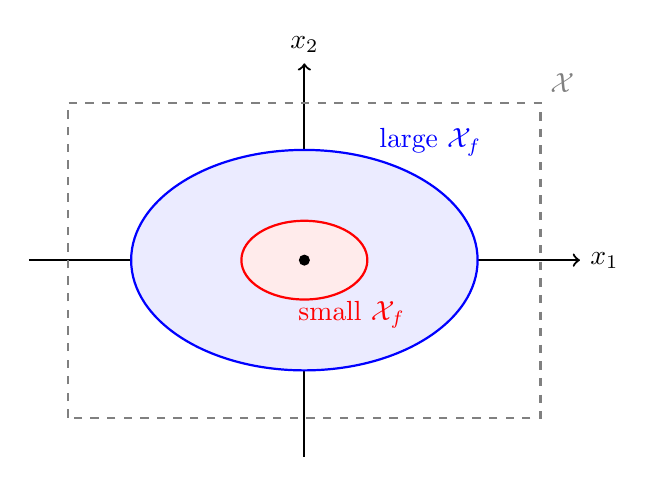
\begin{tikzpicture}[scale=1.0]
		% Axes
		\draw[->, thick] (-3.5,0) -- (3.5,0) node[right] {$x_1$};
		\draw[->, thick] (0,-2.5) -- (0,2.5) node[above] {$x_2$};
		% State constraints (outer box)
		\draw[thick, gray, dashed] (-3,-2) rectangle (3,2);
		\node[gray, anchor=south west] at (3,2) {$\mathcal{X}$};
		% Large terminal set
		\draw[thick, blue, fill=blue!8] (0,0) ellipse (2.2cm and 1.4cm);
		\node[blue, anchor=south] at (1.6,1.2) {large $\mathcal{X}_f$};
		% Small terminal set
		\draw[thick, red, fill=red!8] (0,0) ellipse (0.8cm and 0.5cm);
		\node[red, anchor=north] at (0.6,-0.4) {small $\mathcal{X}_f$};
		% Origin
		\fill (0,0) circle (2pt);
	\end{tikzpicture}
\end{center}

In the figure above, the dashed box is the state constraint set $\mathcal{X}$. With a small $\mathcal{X}_f$ (red), the MPC must work harder to hit the target. With a large $\mathcal{X}_f$ (blue), more initial states lead to feasible problems.

\subsection{Computing $\mathcal{X}_f$ for Multi-State Systems Using MPT3}

For scalar systems, we computed $\mathcal{X}_f$ by hand in the earlier example. For systems with two or more states, the terminal set is a polytope (a region bounded by many linear inequalities), and computing it by hand becomes impractical. The standard approach uses an iterative algorithm:

\begin{enumerate}
	\item Start with the constraint set: $\Omega_0 = \{x \in \mathcal{X} \mid Kx \in \mathcal{U}\}$.
	\item At each iteration, intersect with the pre-image: $\Omega_{i+1} = \Omega_i \cap \{x \mid (A-BK)x \in \Omega_i\}$.
	\item Repeat until $\Omega_{i+1} = \Omega_i$ (the set stops shrinking). This fixed point is the maximal positive invariant set $\mathcal{X}_f$.
\end{enumerate}

The iteration is guaranteed to converge in a finite number of steps for stable closed-loop systems with polytopic constraints.

In MATLAB, the \emph{Multi-Parametric Toolbox 3 (MPT3)}~\cite{Herceg2013} automates this computation. MPT3 is a free toolbox available at \texttt{https://www.mpt3.org}. The following code computes $\mathcal{X}_f$ for a two-state system:

\begin{lstlisting}[language=Matlab, caption={Computing $\mathcal{X}_f$ using MPT3}]
% System matrices
A = [1.2 1; 0 1];
B = [0.5; 1];

% Constraints
umax = 1;
xmax = [5; 5];  % state bounds: -xmax <= x <= xmax

% Step 1: Compute LQR gain and DARE solution
Q = eye(2);
R = 1;
[K_lqr, P_dare] = dlqr(A, B, Q, R);

% Closed-loop matrix under LQR
Acl = A - B*K_lqr;

% Step 2: Define constraint polytopes using MPT3
X = Polyhedron('lb', -xmax, 'ub', xmax);   % state constraints
U = Polyhedron('lb', -umax, 'ub', umax);   % input constraints

% Step 3: Build the closed-loop LTI system
sys = LTISystem('A', Acl);
sys.x.min = -xmax;
sys.x.max = xmax;

% Map input constraints through K: |K*x| <= umax
KPoly = Polyhedron('A', [K_lqr; -K_lqr], 'b', [umax; umax]);

% Step 4: Include input constraint as state constraint, then compute
X_combined = Polyhedron('A', [eye(2); -eye(2); K_lqr; -K_lqr], ...
    'b', [xmax; xmax; umax; umax]);
sys.setDomain('x', X_combined);
Xf = sys.invariantSet();

% Step 5: Visualise
figure;
plot(X, 'color', [0.9 0.9 0.9], 'alpha', 0.3); hold on;
plot(Xf, 'color', 'blue', 'alpha', 0.5);
xlabel('x_1'); ylabel('x_2');
legend('State constraints X', 'Terminal set X_f');
title('Maximal Positive Invariant Set');
\end{lstlisting}

The key function is \texttt{sys.invariantSet()}, which performs the iterative algorithm described above automatically. For the example above, the result is a polytope with several faces (linear inequalities) that can be directly used as the terminal constraint $x_N \in \mathcal{X}_f$ in the MPC formulation.

\begin{notebox}{MPT3 and YALMIP}
	MPT3 uses YALMIP internally, so both toolboxes must be installed. Once $\mathcal{X}_f$ is computed as a \texttt{Polyhedron} object, its half-space representation $H_f x \le h_f$ can be extracted with \texttt{Xf.A} and \texttt{Xf.b}, and added directly to the MPC optimisation as the linear constraint $H_f x_N \le h_f$.
\end{notebox}

\begin{notebox}{Combining MPC with State Estimation}
This chapter assumed that the full state $x_k$ is available for measurement. In practice, only noisy partial measurements $y_k = Cx_k + v_k$ are available, and the state must be estimated using a Kalman filter (Chapter~6). Chapter~8 develops the output-feedback MPC architecture that combines the estimator, a target calculator, and the MPC regulator into a complete control system.
\end{notebox}

% ================================================================
% EXPLICIT MPC
% ================================================================
\section{Explicit MPC: Solving the QP Offline\texorpdfstring{$^{(*)}$}{(*)}}
\label{sec:explicit_mpc}

Throughout this chapter, we solved the MPC optimisation problem \emph{online}: at every sampling instant, a QP solver computes $u_0^*$ before the next sample arrives. For systems with slow dynamics (sampling periods of seconds or longer), this works well. But consider a power converter switching at 100\,kHz, or a micro-electromechanical device with a 10\,$\mu$s control period. At these speeds, even a fast QP solver may not finish in time.

Explicit MPC takes a different approach: solve the MPC problem \emph{once, offline}, for every possible initial state $x_0$. The result is a \emph{piecewise affine} (PWA) control law
\[
u^*(x_0) = K_i\, x_0 + k_i \quad \text{when } x_0 \in \mathcal{R}_i
\]
where $\{\mathcal{R}_1, \mathcal{R}_2, \dots, \mathcal{R}_M\}$ is a partition of the feasible state space into polyhedral regions. At runtime, the controller determines which region contains the current state and evaluates the corresponding affine law. No optimisation, no solver --- just comparisons and arithmetic.

\subsection{Why the Optimal Law Is Piecewise Affine}

The MPC problem from Section~\ref{sec:mpc_formulation} is a QP whose data depend on the initial state $x_0$. The cost is quadratic in the decision variables $u_0, \dots, u_{N-1}$, and all constraints (dynamics, input bounds, state bounds) are linear in both $u$ and $x_0$. This makes MPC a \emph{parametric QP}: a QP parameterised by $x_0$.

At any optimal solution, the KKT conditions partition the constraints into two groups:
\begin{itemize}[nosep]
	\item \textbf{Active} (binding) --- satisfied with equality.
	\item \textbf{Inactive} --- satisfied with strict inequality.
\end{itemize}
For a fixed set of active constraints, the KKT system reduces to linear equations in $(u, x_0)$. Solving gives $u^* = K_i x_0 + k_i$, an affine function of $x_0$. This law remains valid as long as $x_0$ does not move far enough to activate a new constraint or deactivate a current one. The set of all such states forms a convex polyhedron $\mathcal{R}_i$, called a \textit{critical region}.

\begin{defnbox}{Explicit MPC Solution~\cite{Bemporad2002}}
	The optimal control law $u^*(x_0)$ of a linear MPC problem with quadratic cost is a \emph{continuous piecewise affine} function of $x_0$. The state space is partitioned into $M$ convex polyhedral \emph{critical regions} $\{\mathcal{R}_1, \dots, \mathcal{R}_M\}$, and within each region:
	\[
	u^*(x_0) = K_i\, x_0 + k_i, \qquad x_0 \in \mathcal{R}_i.
	\]
	The gains and regions $\{(K_i, k_i, \mathcal{R}_i)\}_{i=1}^M$ are computed offline by solving a \emph{multi-parametric QP (mpQP)}.
\end{defnbox}

Different active-set combinations produce different affine pieces. In one region the input constraint may be active; in an adjacent region, a state constraint takes over. The boundaries between regions are the hyperplanes where these transitions occur.

\subsection{Worked Example: Scalar System}

We return to the scalar system from Section~\ref{subsec:terminal_set_scalar}:
\[
x_{k+1} = 1.2\, x_k + u_k, \qquad |u_k| \le 1,
\]
with $Q = 1$, $R = 1$, and $N = 1$. The DARE gives $P \approx 1.95$, and the LQR gain is $K = 1.2P/(1+P) \approx 0.79$.

\begin{examplebox}{Explicit MPC for the Scalar System}

The MPC problem for a given initial state $x_0$ is:
\[
\min_{u_0}\; x_0^2 + u_0^2 + 1.95\,(1.2\, x_0 + u_0)^2
\qquad \text{s.t.} \quad -1 \le u_0 \le 1.
\]

\solution

Expanding the cost:
\[
J(u_0) = \underbrace{(1 + 1.44\,P)}_{= 3.81}\, x_0^2 + 2 \cdot 1.2\,P\, x_0\, u_0 + \underbrace{(1 + P)}_{= 2.95}\, u_0^2.
\]
This is a quadratic in $u_0$ with positive curvature. The unconstrained minimum is:
\[
\frac{\mathrm{d}J}{\mathrm{d}u_0} = 0 \quad\Longrightarrow\quad
u_0^{\text{unc}} = -\frac{1.2\,P}{1 + P}\, x_0 = -K\, x_0 \approx -0.79\, x_0.
\]
The constraint $|u_0| \le 1$ becomes active when $|Kx_0| = 1$, i.e.\ when $|x_0| = 1/K \approx 1.26$.

Three cases arise depending on where $x_0$ sits:

\textbf{Case 1: $x_0 \le -1.26$.} The unconstrained optimum $-Kx_0$ exceeds $+1$, so the upper bound constraint is active. The optimal input is $u^* = +1$ (full positive force to pull the state back).

\textbf{Case 2: $-1.26 \le x_0 \le 1.26$.} The unconstrained optimum satisfies $|u_0| \le 1$. No constraint is active. The optimal input is $u^* = -0.79\,x_0$ (identical to LQR).

\textbf{Case 3: $x_0 \ge 1.26$.} The unconstrained optimum $-Kx_0$ falls below $-1$, so the upper bound constraint is active. The optimal input is $u^* = -1$ (full negative force).

The explicit law is:
\[
u^*(x_0) = \begin{cases}
	+1 & x_0 \le -1.26 \quad (\mathcal{R}_1) \\[3pt]
	-0.79\, x_0 & |x_0| \le 1.26 \quad (\mathcal{R}_2) \\[3pt]
	-1 & x_0 \ge 1.26 \quad (\mathcal{R}_3)
\end{cases}
\]

\end{examplebox}

Figure~\ref{fig:explicit_scalar_pwa} plots this law. In $\mathcal{R}_2$, the controller behaves identically to LQR. In $\mathcal{R}_1$ and $\mathcal{R}_3$, the actuator is saturated. The breakpoints at $x_0 = \pm 1/K$ mark where the input constraint switches from inactive to active.

\begin{figure}[ht]
	\centering
	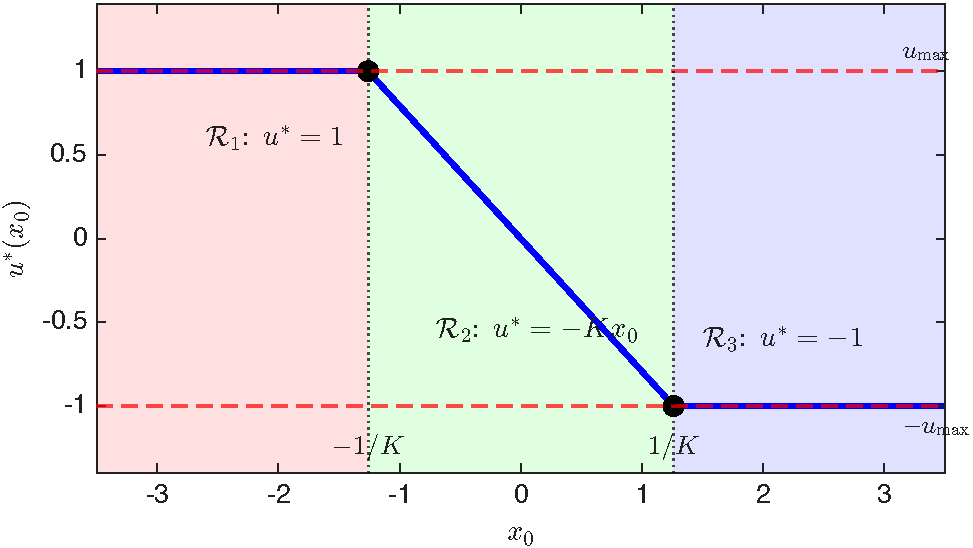
\includegraphics[width=0.85\textwidth]{Figures/fig_explicit_scalar_pwa.pdf}
	\caption{Explicit MPC law $u^*(x_0)$ for the scalar system with $|u| \le 1$, $N = 1$, $Q = R = 1$. The three critical regions correspond to: lower input constraint active ($\mathcal{R}_1$), unconstrained ($\mathcal{R}_2$), and upper constraint active ($\mathcal{R}_3$). Online evaluation requires two comparisons and one multiplication.}
	\label{fig:explicit_scalar_pwa}
\end{figure}

At runtime, the entire controller reduces to:
\begin{lstlisting}[language=Matlab, numbers=none]
if x0 <= -1.26,      u = 1;
elseif x0 >= 1.26,   u = -1;
else,                 u = -0.79 * x0;
end
\end{lstlisting}
Two comparisons and one multiply. This executes in nanoseconds on any microcontroller --- no QP solver, no YALMIP, no operating system required.

\subsection{Multi-State Systems: MPT3 Workflow}

For systems with two or more states, the critical regions are polytopes in $\mathbb{R}^n$ and must be computed algorithmically. MPT3~\cite{Herceg2013} automates the entire workflow: define the system, set up the MPC problem, and call \texttt{toExplicit()}.

We use the same double integrator as the terminal set example:
\[
A = \begin{bmatrix} 1.2 & 1 \\ 0 & 1 \end{bmatrix}, \quad B = \begin{bmatrix} 0.5 \\ 1 \end{bmatrix}, \quad |u_k| \le 1, \quad |x_{i,k}| \le 5,
\]
with $Q = I_2$, $R = 1$, $N = 5$, and the DARE terminal cost $P$.

\begin{lstlisting}[language=Matlab, caption={Computing Explicit MPC via MPT3}]
% 1. System definition
A = [1.2 1; 0 1];  B = [0.5; 1];
sys = LTISystem('A', A, 'B', B);

% 2. Constraints
sys.x.min = [-5; -5];   sys.x.max = [5; 5];
sys.u.min = -1;          sys.u.max = 1;

% 3. Cost: Q, R, terminal cost P from DARE
Q = eye(2);  R = 1;  N = 5;
[~, P] = dlqr(A, B, Q, R);
sys.x.penalty  = QuadFunction(Q);
sys.u.penalty  = QuadFunction(R);
sys.x.with('terminalPenalty');
sys.x.terminalPenalty = QuadFunction(P);

% 4. Build online MPC, then convert to explicit
mpc_online = MPCController(sys, N);
empc = mpc_online.toExplicit();
fprintf('Critical regions: %d\n', empc.nr);

% 5. Plot the polyhedral partition
figure;
empc.partition.plot();
xlabel('x_1');  ylabel('x_2');
title('Explicit MPC: Critical Regions');

% 6. Evaluate at runtime --- table lookup, no solver
x_now = [3; -1];
u_star = empc.evaluate(x_now);
fprintf('u*(x0) = %.4f\n', u_star);
\end{lstlisting}

Figure~\ref{fig:explicit_regions_2d} shows the resulting partition. Each coloured polygon is one critical region with its own affine gain $(K_i, k_i)$. The partition tiles the feasible state space without gaps or overlaps. At runtime, the controller performs a \emph{point-location query} --- testing which region contains the current state --- and evaluates $u^* = K_i x + k_i$.

\begin{figure}[ht]
	\centering
	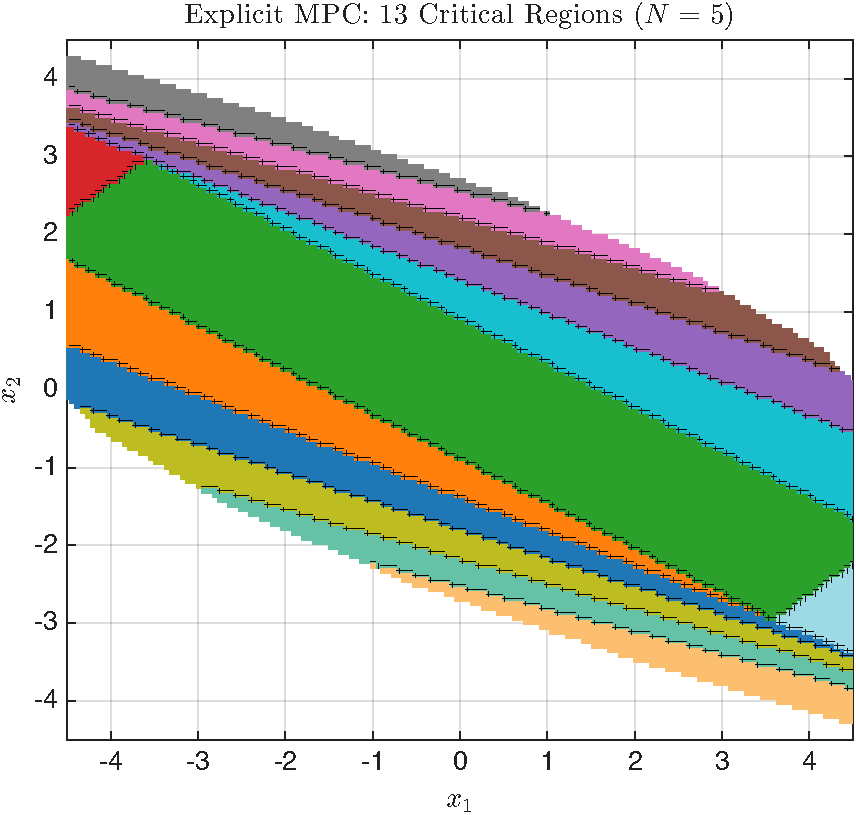
\includegraphics[width=0.75\textwidth]{Figures/fig_explicit_regions_2d.pdf}
	\caption{Polyhedral partition of the state space for the double integrator under explicit MPC with $N = 5$. Each coloured region has a distinct affine feedback gain. The partition is computed once offline; online control reduces to identifying which region contains the current state.}
	\label{fig:explicit_regions_2d}
\end{figure}

The explicit and online controllers produce \emph{identical} results --- explicit MPC is not an approximation. To verify, we simulate both controllers in closed loop from the same initial condition $x_0 = [4,\; -1]^\top$:

\begin{lstlisting}[language=Matlab, caption={Verifying explicit vs.\ online MPC equivalence}]
T_sim = 30;  x0 = [4; -1];
x_on = zeros(2, T_sim+1);  x_on(:,1) = x0;
x_ex = x_on;
u_on = zeros(1, T_sim);    u_ex = u_on;

for t = 1:T_sim
    u_on(t) = mpc_online.evaluate(x_on(:,t));   % solves QP
    x_on(:,t+1) = A*x_on(:,t) + B*u_on(t);

    u_ex(t) = empc.evaluate(x_ex(:,t));          % table lookup
    x_ex(:,t+1) = A*x_ex(:,t) + B*u_ex(t);
end
fprintf('Max |u_online - u_explicit| = %.2e\n', max(abs(u_on-u_ex)));
% Output: 1.30e-09 (numerical precision only)
\end{lstlisting}

Figure~\ref{fig:explicit_online_vs_explicit} confirms the equivalence. The state and input trajectories of both controllers overlap completely --- the red dashed line (explicit) sits exactly on top of the blue solid line (online) in all three subplots. The maximum difference in control input is $1.3 \times 10^{-9}$, i.e.\ zero to machine precision.

\begin{figure}[ht]
	\centering
	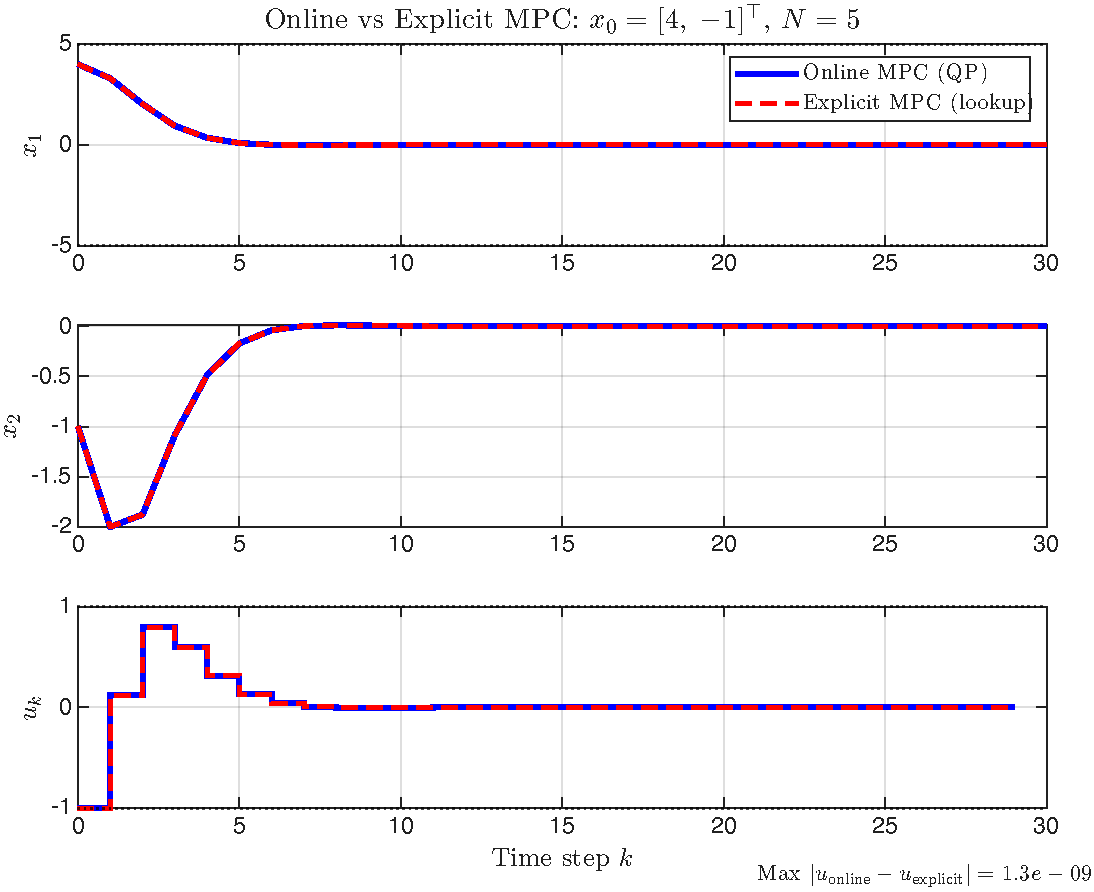
\includegraphics[width=0.9\textwidth]{Figures/fig_explicit_online_vs_explicit.pdf}
	\caption{Closed-loop comparison of online MPC (QP solved at each step) and explicit MPC (PWA lookup table) for the double integrator with $N = 5$, $x_0 = [4,\; -1]^\top$. The trajectories are indistinguishable: explicit MPC reproduces the online solution exactly.}
	\label{fig:explicit_online_vs_explicit}
\end{figure}

\subsection{The Price: Complexity Growth}

The number of critical regions $M$ determines both the offline computation time and the online storage. Each region requires storing one gain matrix $K_i \in \mathbb{R}^{n_u \times n_x}$, one offset $k_i \in \mathbb{R}^{n_u}$, and a set of half-space inequalities defining $\mathcal{R}_i$. As the system dimension, number of constraints, or prediction horizon grows, $M$ can increase rapidly.

\begin{alertbox}{Curse of dimensionality}
	The number of critical regions grows combinatorially with the problem size:
	\begin{itemize}[nosep]
		\item $n_x \le 3$, moderate $N$: tens to hundreds of regions. Practical for most embedded platforms.
		\item $n_x = 4$--$5$: thousands of regions. Feasible with care (storage in the megabyte range).
		\item $n_x \ge 6$: tens of thousands of regions or more. The offline computation may take hours and the resulting lookup table may exceed embedded memory.
	\end{itemize}
	For large systems, online QP solvers or first-order optimisation methods are preferable.
\end{alertbox}

\begin{summarybox}{Explicit MPC: When to Use It}
	\begin{center}
		\renewcommand{\arraystretch}{1.3}
		\begin{tabular}{p{0.44\textwidth} p{0.44\textwidth}}
			\toprule
			\textbf{Use explicit MPC when \dots} & \textbf{Use online MPC when \dots} \\
			\midrule
			Sampling period is very short ($\mu$s) & Sampling period allows solver time (ms--s) \\
			Few states ($n_x \le 4$) & Many states ($n_x \ge 5$) \\
			No solver available on hardware & QP solver library available \\
			Deterministic worst-case timing needed & Average-case timing acceptable \\
			Model and constraints are fixed & Model or constraints change at runtime \\
			\bottomrule
		\end{tabular}
	\end{center}
\end{summarybox}

% ================================================================
% REFERENCE TRACKING MPC
% ================================================================
\section{Reference Tracking MPC\texorpdfstring{$^{(*)}$}{(*)}}
\label{sec:tracking_mpc}

Chapters~7 and~8 focus on \emph{regulation}: driving the state to the origin, or to a constant setpoint via offset-free MPC. Many applications require the system to follow a \emph{time-varying reference trajectory} $\{x^r_k, u^r_k\}_{k=0}^{\infty}$ --- a robotic arm tracing a contour, a vehicle following a lane, or a satellite executing an orbital manoeuvre.

This section extends the MPC framework to handle trajectory tracking, including nonlinear systems for which the linearisation changes along the reference path.

\subsection{From Regulation to Tracking}

In a regulation problem, the cost penalises the state itself:
\[
J = \sum_{k=0}^{N-1} \bigl(x_k^\top Q\, x_k + u_k^\top R\, u_k\bigr) + x_N^\top P\, x_N.
\]
For tracking, we penalise the \emph{deviation} from the reference. Define:
\[
\delta x_k = x_k - x^r_k, \qquad \delta u_k = u_k - u^r_k,
\]
where $x^r_k$ and $u^r_k$ are the reference state and input at time $k$. The tracking cost becomes:
\[
J_{\text{track}} = \sum_{k=0}^{N-1} \bigl(\delta x_k^\top Q\, \delta x_k + \delta u_k^\top R\, \delta u_k\bigr) + \delta x_N^\top P\, \delta x_N.
\]

\begin{notebox}{Tracking vs.\ Offset-Free MPC (Chapter~\ref{chap:output_fb_mpc})}
	The offset-free MPC of Chapter~\ref{chap:output_fb_mpc} tracks a \emph{constant} setpoint by augmenting the model with a disturbance estimator and a target calculator. Here we address a fundamentally different problem: the reference changes at every time step, the full reference trajectory is assumed known over the prediction horizon, and no disturbance estimation is needed.
\end{notebox}

For a \emph{linear time-invariant} system $x_{k+1} = Ax_k + Bu_k$ whose reference satisfies the same dynamics ($x^r_{k+1} = Ax^r_k + Bu^r_k$), subtracting yields:
\[
\delta x_{k+1} = A\,\delta x_k + B\,\delta u_k.
\]
The tracking problem then reduces to a standard regulation problem in the deviation variables $(\delta x, \delta u)$, with the same matrices $A$ and $B$. Input constraints $u_{\min} \le u_k \le u_{\max}$ translate to:
\[
u_{\min} - u^r_k \;\le\; \delta u_k \;\le\; u_{\max} - u^r_k.
\]
The constraint bounds shift at each prediction step --- the QP structure is identical but the data changes.

\subsection{Nonlinear Tracking via Successive Linearisation}

When the plant is nonlinear,
\[
x_{k+1} = f(x_k, u_k),
\]
the deviation dynamics are no longer exactly linear. A standard approach is to \emph{linearise around the reference trajectory} at each prediction step $k$:
\begin{align*}
	A_k &= \left.\frac{\partial f}{\partial x}\right|_{x^r_k,\, u^r_k}, &
	B_k &= \left.\frac{\partial f}{\partial u}\right|_{x^r_k,\, u^r_k}.
\end{align*}
The linearised deviation dynamics become \emph{time-varying}:
\[
\delta x_{k+1} \approx A_k\,\delta x_k + B_k\,\delta u_k.
\]
At each MPC step, we solve a QP over the deviation variables with these time-varying matrices. The resulting optimisation is still a convex QP --- only the constraint and cost data change from step to step.

\begin{alertbox}{Successive Linearisation Is Not Globally Optimal}
	Each QP uses a first-order approximation of $f$ around the reference. If the actual state deviates significantly from the reference, the linearisation error grows. For large deviations, iterating the linearisation (re-linearising around the predicted trajectory rather than the reference) improves accuracy at the cost of solving multiple QPs per step. This idea---\emph{successive convexification}---is developed formally in Chapter~\ref{chap:nmpc}, alongside the full nonlinear MPC framework.
\end{alertbox}

\subsection{Application: Path Following for a Mobile Robot}

We apply tracking MPC to a nonholonomic mobile robot --- a standard platform in robotics whose motion constraints make it a natural testbed for nonlinear tracking.

\subsubsection*{The Unicycle Model}

A differential-drive robot moving on a plane has state $x = [p_x,\; p_y,\; \theta]^\top$ (position and heading) and input $u = [v,\; \omega]^\top$ (linear speed and angular rate). The continuous-time kinematics are:
\begin{align*}
	\dot{p}_x &= v\,\cos\theta, &
	\dot{p}_y &= v\,\sin\theta, &
	\dot{\theta} &= \omega.
\end{align*}
The system is nonholonomic: it cannot move sideways. Despite having three state variables, only two inputs are available, and the velocity direction is coupled to the heading through $\cos\theta$ and $\sin\theta$.

\textbf{Discretisation.} Applying Forward Euler with sampling period $T_s$:
\begin{equation*}
	\underbrace{\begin{bmatrix} p_{x,k+1} \\ p_{y,k+1} \\ \theta_{k+1} \end{bmatrix}}_{x_{k+1}}
	= \underbrace{\begin{bmatrix} p_{x,k} + T_s\, v_k \cos\theta_k \\ p_{y,k} + T_s\, v_k \sin\theta_k \\ \theta_k + T_s\, \omega_k \end{bmatrix}}_{f(x_k, u_k)}.
\end{equation*}

\textbf{Jacobians.} At a reference point $(x^r_k, u^r_k)$ with $\theta^r_k$ and $v^r_k$:
\[
A_k = \begin{bmatrix} 1 & 0 & -T_s\, v^r_k \sin\theta^r_k \\ 0 & 1 & T_s\, v^r_k \cos\theta^r_k \\ 0 & 0 & 1 \end{bmatrix}, \qquad
B_k = \begin{bmatrix} T_s \cos\theta^r_k & 0 \\ T_s \sin\theta^r_k & 0 \\ 0 & T_s \end{bmatrix}.
\]
Both matrices change along the reference path because $\theta^r_k$ and $v^r_k$ vary with $k$.

\subsubsection*{Circular Reference Trajectory}

The robot follows a circle of radius $R$ at constant speed. The reference trajectory is:
\[
x^r_k = \begin{bmatrix} R\cos(\omega_{\text{ref}}\, k T_s) \\ R\sin(\omega_{\text{ref}}\, k T_s) \\ \omega_{\text{ref}}\, k T_s + \tfrac{\pi}{2} \end{bmatrix}, \qquad
u^r_k = \begin{bmatrix} R\,\omega_{\text{ref}} \\ \omega_{\text{ref}} \end{bmatrix},
\]
where $\omega_{\text{ref}}$ is the angular rate around the circle. The reference heading is tangent to the circle (offset by $\pi/2$ from the radial direction), and the reference speed is $v^r = R\,\omega_{\text{ref}}$.

\subsubsection*{The Tracking MPC Problem}

At each time step $t$, given the current state $x_t$ and the known reference $\{x^r_{t+k}, u^r_{t+k}\}_{k=0}^{N}$, we solve:
\begin{align*}
	\min_{\delta u_0, \dots, \delta u_{N-1}} \quad & \sum_{k=0}^{N-1} \bigl(\delta x_k^\top Q\,\delta x_k + \delta u_k^\top R\,\delta u_k\bigr) + \delta x_N^\top Q\,\delta x_N \\[4pt]
	\text{s.t.} \quad
	& \delta x_0 = x_t - x^r_t \hspace{5.6cm} \text{(Initialisation)} \\
	& \delta x_{k+1} = A_k\,\delta x_k + B_k\,\delta u_k, \quad k = 0, \dots, N{-}1 \hspace{0.2cm} \text{(Linearised Dynamics)} \\
	& u_{\min} - u^r_{t+k} \le \delta u_k \le u_{\max} - u^r_{t+k} \hspace{1.95cm} \text{(Actuator Limits)}
\end{align*}
The first optimal deviation $\delta u_0^*$ is applied: $u_t = u^r_t + \delta u_0^*$.

\subsubsection*{MATLAB Implementation}

The following code implements the complete tracking MPC loop for the unicycle on a circular path.

\begin{lstlisting}[language=Matlab, caption={Tracking MPC for a nonholonomic mobile robot following a circular path.}]
% 1. Parameters
Ts = 0.1;  R_c = 3;  w_ref = 0.5;
v_ref = R_c * w_ref;  N = 15;  T_sim = 150;
Q = diag([10, 10, 2]);  Rw = diag([0.5, 0.5]);
v_min = 0;  v_max = 2.5;  w_min = -1.5;  w_max = 1.5;

% 2. Reference trajectory
t_all = (0:T_sim+N) * Ts;
xr = [R_c*cos(w_ref*t_all); R_c*sin(w_ref*t_all);
      w_ref*t_all + pi/2];
ur = repmat([v_ref; w_ref], 1, T_sim+N);

% 3. Nonlinear dynamics (Forward Euler)
f_nl = @(x,u) x + Ts*[u(1)*cos(x(3)); u(1)*sin(x(3)); u(2)];

% 4. Closed-loop simulation
x0 = [R_c+1.5; 1.0; pi/2+0.3];
x_log = zeros(3, T_sim+1);  x_log(:,1) = x0;
u_log = zeros(2, T_sim);

for t = 1:T_sim
    dx = sdpvar(3, N+1, 'full');
    du = sdpvar(2, N, 'full');

    con = [dx(:,1) == x_log(:,t) - xr(:,t)];
    obj = 0;
    for k = 1:N
        th_r = xr(3, t+k-1);  vr_k = ur(1, t+k-1);
        Ak = [1, 0, -Ts*vr_k*sin(th_r);
              0, 1,  Ts*vr_k*cos(th_r);
              0, 0,  1];
        Bk = [Ts*cos(th_r), 0; Ts*sin(th_r), 0; 0, Ts];

        con = [con, dx(:,k+1) == Ak*dx(:,k) + Bk*du(:,k)];
        con = [con, v_min-ur(1,t+k-1) <= du(1,k) <= v_max-ur(1,t+k-1)];
        con = [con, w_min-ur(2,t+k-1) <= du(2,k) <= w_max-ur(2,t+k-1)];
        obj = obj + dx(:,k)'*Q*dx(:,k) + du(:,k)'*Rw*du(:,k);
    end
    obj = obj + dx(:,N+1)'*Q*dx(:,N+1);

    optimize(con, obj, sdpsettings('verbose',0,'solver','quadprog'));
    u_log(:,t) = ur(:,t) + value(du(:,1));
    x_log(:,t+1) = f_nl(x_log(:,t), u_log(:,t));
end
\end{lstlisting}

\begin{alertbox}{Performance Note}
The code above calls \texttt{optimize} inside the simulation loop because the Jacobians $A_k$, $B_k$ change at every prediction step. This forces YALMIP to re-parse the problem at each time step, which is orders of magnitude slower than using \texttt{optimizer}. For real-time applications, one should either parameterise the Jacobians as \texttt{sdpvar} parameters or use CasADi's parametric NLP interface.
\end{alertbox}

\subsubsection*{Results}

Figure~\ref{fig:tracking_mpc_robot} shows the simulation with parameters $T_s = 0.1$\,s, $R = 3$\,m, $\omega_{\text{ref}} = 0.5$\,rad/s (one lap $\approx 12.6$\,s), $N = 15$, $Q = \operatorname{diag}(10,10,2)$, $R = \operatorname{diag}(0.5, 0.5)$.

The robot starts at $(4.5,\, 1.0)$ with heading $\theta_0 = \pi/2 + 0.3$ --- displaced from the reference circle. Within the first two seconds, the tracking MPC steers the robot onto the circular path and maintains close tracking for the remainder of the simulation. The triangular markers indicate the robot's position and heading at selected time steps.

The position errors (top-right subplot) show a transient phase during which the MPC corrects the initial offset, followed by near-zero steady-state tracking. The control inputs (bottom-right subplot) remain within the actuator limits $v \in [0,\, 2.5]$\,m/s and $\omega \in [-1.5,\, 1.5]$\,rad/s throughout.

\begin{figure}[ht]
	\centering
	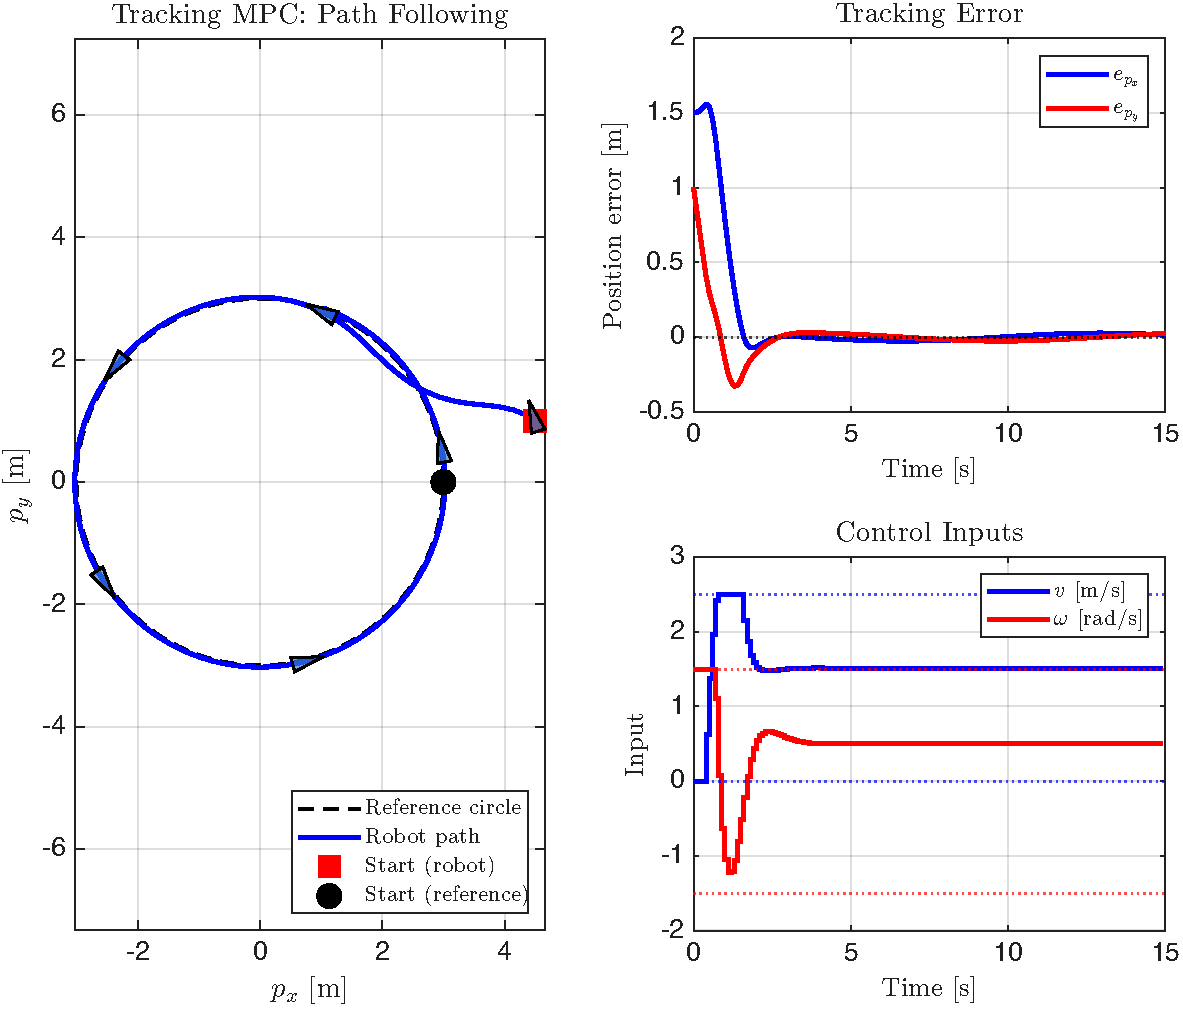
\includegraphics[width=0.95\textwidth]{Figures/fig_tracking_mpc_robot.pdf}
	\caption{Tracking MPC for a nonholonomic mobile robot following a circular path ($R = 3$\,m, $\omega_{\text{ref}} = 0.5$\,rad/s). Left: the robot (blue) converges onto the reference circle (dashed) from a displaced initial position. Top-right: position tracking errors decay to near zero. Bottom-right: linear speed $v$ and angular rate $\omega$ respect the actuator limits.}
	\label{fig:tracking_mpc_robot}
\end{figure}

\begin{summarybox}{Reference Tracking MPC}
	\begin{enumerate}[nosep]
		\item Define the reference trajectory $\{x^r_k, u^r_k\}$ over the prediction horizon.
		\item Compute deviation variables: $\delta x_k = x_k - x^r_k$, $\delta u_k = u_k - u^r_k$.
		\item For nonlinear systems, linearise $f$ around the reference at each prediction step to obtain time-varying $(A_k, B_k)$.
		\item Solve a QP in $(\delta x, \delta u)$ with shifted input constraints $u_{\min} - u^r_k \le \delta u_k \le u_{\max} - u^r_k$.
		\item Apply $u_t = u^r_t + \delta u_0^*$ to the plant. Shift the horizon and repeat.
	\end{enumerate}
\end{summarybox}

\section*{Chapter Summary}
\begin{itemize}
    \item Constrained MPC formulates the control problem as a finite-horizon optimisation with explicit inequality constraints on states and inputs.
    \item The MPC optimisation is cast as a quadratic program (QP) by substituting the predicted state trajectory in terms of the initial state and the input sequence.
    \item YALMIP provides a convenient MATLAB interface for defining decision variables, constraints, and objectives, and dispatching the resulting QP to a solver.
    \item A terminal cost term, chosen as the solution to the discrete algebraic Riccati equation (DARE), approximates the infinite-horizon cost beyond the prediction window.
    \item A terminal constraint set ensures that the state at the end of the horizon lies in a controlled-invariant region, guaranteeing recursive feasibility.
    \item Closed-loop stability is established via a Lyapunov argument showing that the optimal cost decreases at each time step under the receding-horizon policy.
    \item Explicit MPC pre-computes the optimal control law offline as a piecewise affine function of the state, enabling real-time implementation without online QP solves.
    \item Reference tracking MPC reformulates the problem in terms of deviation variables around a target steady state, allowing the controller to follow time-varying setpoints.
\end{itemize}

\section*{Exercises}
\begin{enumerate}

\item Consider the scalar system
\[
x_{k+1} = 1.5\, x_k + u_k
\]
with weighting matrices $Q = 1$, $R = 2$, and a prediction horizon $N = 2$.
\begin{enumerate}
	\item Write out the predicted states $x_1$ and $x_2$ as functions of $x_0$ and the decision variables $u_0, u_1$.
	\item Using these expressions, eliminate the states from the cost function
	\[
	J = x_2^\top Q_N\, x_2 + \sum_{k=0}^{1}\bigl(x_k^\top Q\, x_k + u_k^\top R\, u_k\bigr)
	\]
	(set $Q_N = Q$ for simplicity) and express $J$ in the standard quadratic form
	\[
	J = u^\top H\, u + 2\, x_0^\top f^\top u + \text{const.}
	\]
	where $u = [u_0 \;\; u_1]^\top$. State the matrices $H$ and $f$ explicitly.
\end{enumerate}

\item For the system
\[
x_{k+1} = 1.2\, x_k + u_k, \qquad Q = 1, \quad R = 0.5, \quad N = 1, \quad Q_N = Q,
\]
with no constraints and an initial condition $x_0 = 3$:
\begin{enumerate}
	\item Show that the MPC optimisation at $k = 0$ reduces to a single-variable unconstrained quadratic minimisation in $u_0$.
	\item Find the optimal input $u_0^\star$ and the resulting next state $x_1$.
	\item Explain why only $u_0^\star$ is applied to the plant and what happens at the next sampling instant under the receding horizon principle.
\end{enumerate}

\item Consider the same system as in Exercise~2, but now add the input constraint $-1 \le u_k \le 1$.
\begin{enumerate}
	\item For $x_0 = 3$, determine whether the unconstrained optimum $u_0^\star$ from Exercise~2 violates the constraint. If so, find the constrained optimum.
	\item Repeat for $x_0 = 10$. Simulate the closed-loop response for several steps by applying the receding horizon strategy with $N = 1$. Does the state converge to the origin?
	\item Determine (analytically or by trial) the largest initial condition $|x_0|$ for which the MPC problem with $N = 1$ and $-1 \le u_k \le 1$ remains feasible. What happens if $x_0$ exceeds this value?
\end{enumerate}

\item Consider a double integrator in discrete time:
\[
A = \begin{bmatrix} 1 & 1 \\ 0 & 1 \end{bmatrix}, \qquad B = \begin{bmatrix} 0.5 \\ 1 \end{bmatrix},
\]
with $Q = I_2$, $R = 1$, $Q_N = Q$, input constraint $-1 \le u_k \le 1$, and initial condition $x_0 = [4 \;\; 0]^\top$.
\begin{enumerate}
	\item Using YALMIP (or by hand for $N = 2$), solve the MPC problem for horizons $N = 2, 5, 10, 20$ and record the first optimal input $u_0^\star$ in each case.
	\item Simulate the closed-loop response for each horizon length over $30$ time steps. Plot the state trajectories and input sequences.
	\item Discuss how $N$ affects the speed of convergence, constraint activity, and computational cost. What is the minimum $N$ for which the closed-loop system appears stable?
\end{enumerate}

\item Return to the scalar system
\[
x_{k+1} = 1.2\, x_k + u_k, \qquad -1 \le u_k \le 1,
\]
with $Q = 1$, $R = 10$, and $x_0 = 4$.
\begin{enumerate}
	\item Solve the discrete algebraic Riccati equation to obtain the terminal cost weight $P$.
	\item Simulate the closed-loop system under MPC with $N = 3$ and $Q_N = Q$ (no terminal cost correction). Repeat with $Q_N = P$. Compare the convergence rates.
	\item Explain, using the concept of the infinite-horizon cost-to-go, why adding the terminal cost $P$ improves performance even though the horizon $N$ remains short.
	\item For the case $Q_N = P$, under what conditions is the terminal cost a valid approximation of the true cost-to-go beyond the horizon? State the role of the terminal set $\mathcal{X}_f$ and the terminal control law $u = -Kx$ in a rigorous stability proof.
\end{enumerate}

\item A control engineer designs an MPC controller for a chemical reactor modelled as
\[
x_{k+1} = A x_k + B u_k, \qquad x_k \in \mathbb{R}^3, \quad u_k \in \mathbb{R}^2,
\]
with state constraints $x_{\min} \le x_k \le x_{\max}$ representing safety limits and input constraints $u_{\min} \le u_k \le u_{\max}$ representing valve positions.
\begin{enumerate}
	\item The engineer observes that the MPC solver returns an infeasibility warning at certain operating points. List three possible causes of infeasibility and, for each, suggest a practical remedy.
	\item The engineer proposes softening the state constraints by introducing slack variables $\epsilon_k \ge 0$ and replacing $x_{\min} \le x_k \le x_{\max}$ with $x_{\min} - \epsilon_k \le x_k \le x_{\max} + \epsilon_k$, adding a penalty $\rho \|\epsilon_k\|^2$ to the cost. Explain the trade-off involved in choosing $\rho$ and why input constraints should generally \emph{not} be softened.
	\item The engineer is considering two design choices: (i)~a short horizon $N = 5$ with the DARE terminal cost $Q_N = P$, and (ii)~a long horizon $N = 50$ with $Q_N = Q$. Discuss the advantages and disadvantages of each choice in terms of closed-loop stability, computational load, and robustness to model uncertainty.
\end{enumerate}

\item \textbf{(Explicit MPC)} Consider the scalar system $x_{k+1} = 1.5\,x_k + u_k$ with $|u_k| \le 1$, $Q = 1$, $R = 0.5$.
\begin{enumerate}
	\item Solve the DARE to find $P$. Compute the LQR gain $K$ and the breakpoint $x_{\text{bp}} = 1/K$.
	\item For $N = 1$, derive the explicit MPC law $u^*(x_0)$. State each critical region and its affine law. Verify that the law is continuous at the breakpoints.
	\item Now add a state constraint $|x_k| \le 3$. For $N = 1$, the constraint $|1.5\,x_0 + u_0| \le 3$ introduces additional breakpoints. Find them and sketch the new $u^*(x_0)$.
	\item For $N = 2$ with input constraints only ($|u_k| \le 1$, no state constraint), how many possible active-set combinations exist? Use MATLAB to compute and plot $u_0^*(x_0)$. How many critical regions arise?
	\item If you have MPT3 installed, compute the explicit controller for the double integrator from Exercise~4 with horizons $N = 3, 5, 10$. Report the number of critical regions for each case and comment on the growth rate.
\end{enumerate}

\end{enumerate}

